\section{Mô tả ca sử dụng}

Phần này đi sâu vào mô tả chi tiết các ca sử dụng (use cases) chính của hệ thống VieVu. Mục tiêu là làm rõ cách thức người dùng tương tác với hệ thống để thực hiện các chức năng đã được xác định trong phần đặc tả yêu cầu. Mỗi ca sử dụng sẽ được trình bày theo một cấu trúc chuẩn hóa, bao gồm các yếu tố như tác nhân (actor), điều kiện tiên quyết (preconditions), luồng sự kiện chính (main flow), các luồng thay thế (alternative flows), và điều kiện kết thúc (postconditions). Việc phân tích và mô tả các ca sử dụng này không chỉ đảm bảo rằng tất cả các yêu cầu chức năng được bao phủ mà còn cung cấp một góc nhìn chi tiết về hoạt động của hệ thống từ quan điểm của người dùng cuối.

\subsection{Ca sử dụng đăng ký}
\vspace{0.5cm}


\noindent 
\begin{tabularx}{\linewidth}{| l | X |} 
\hline 
\textbf{Mô tả} & Cho phép người dùng tạo một tài khoản trên ứng dụng để sử dụng các chức năng. \\ 
\hline 
\textbf{Luồng cơ bản} & 1. Người dùng truy cập màn hình đăng ký tài khoản. \newline
                       2. Ứng dụng hiển thị giao diện đăng ký tài khoản, yêu cầu người dùng nhập thông tin. \newline
                       3. Người dùng điền tên, email và mật khẩu của tài khoản muốn đăng ký. \newline
                       4. Người dùng nhấn đăng ký để hoàn thành quá trình. \newline
                       5. Hệ thống kiểm tra thông tin người dùng để trả về thông báo phù hợp và điều hướng người dùng đến màn hình điền khảo sát sở thích. \\ 
\hline 
\textbf{Luồng thay thế} &
                       - Nếu có lỗi tại server, hệ thống sẽ không lưu lại thông tin đã nhập vào. \newline
                       - Nếu thông tin nhập vào không hợp lệ sẽ thông báo lỗi để người dùng nhập lại. \\ 
\hline 
\textbf{Tiền điều kiện} & - Màn hình đăng ký đã hiển thị thành công trên ứng dụng. \newline
                       - Tài khoản email đúng định dạng và chưa được đăng ký trước đây. \\ 
\hline 
\textbf{Hậu điều kiện} & - Người đã đăng ký tài khoản có thể sử dụng nó để đăng nhập và thực hiện các chức năng với quyền hạn tương ứng. \newline
                       - Một hồ sơ người dùng và thông tin về sở thích được tạo và có thể được chỉnh sửa. \\ 
\hline 
\textbf{Yêu cầu phi chức năng} & Hệ thống xử lý đăng ký không quá 2s \\ 
\hline 
\end{tabularx}

\vspace{0.8cm}

\noindent 
\begin{tabular}{| c | c |}
    \hline
    \textbf{Biểu đồ hoạt động} & \textbf{Quan hệ} \\ 
    \hline
    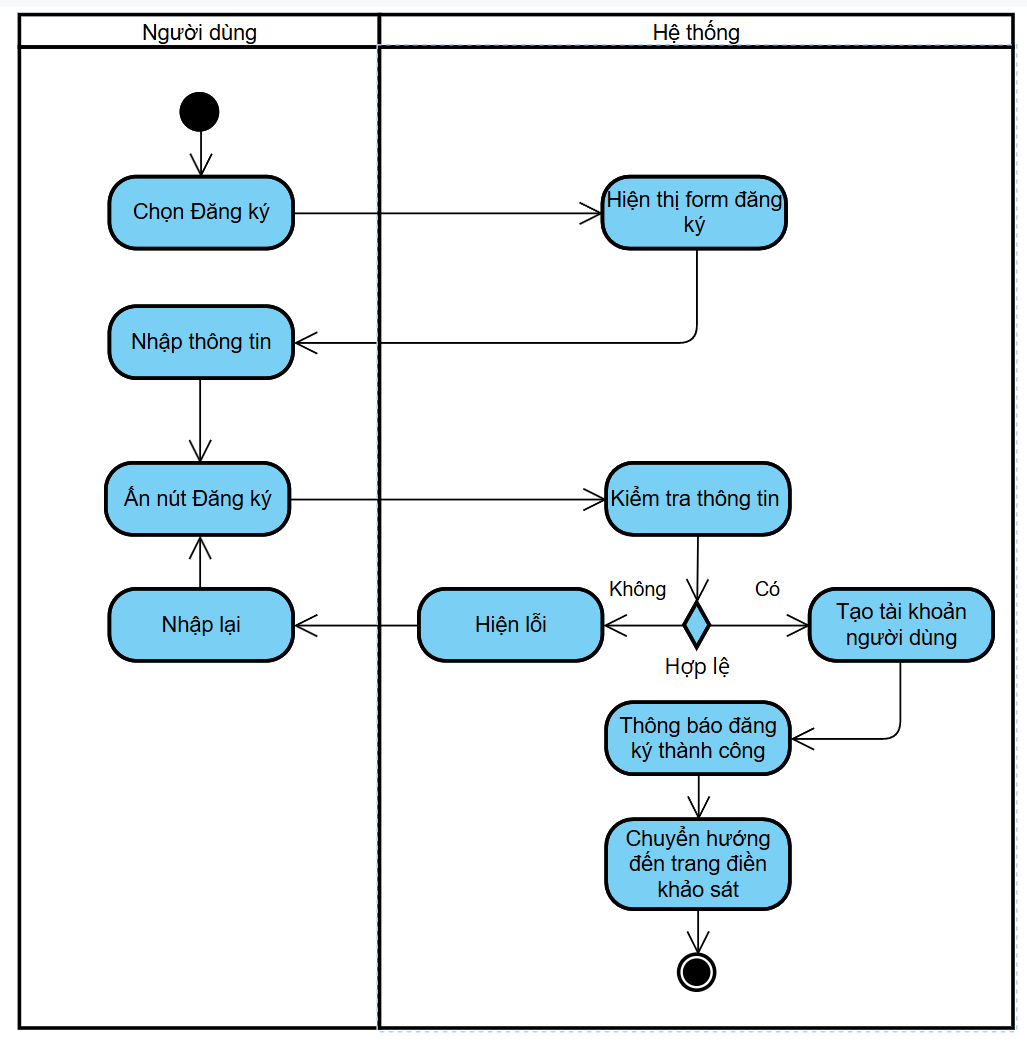
\includegraphics[width=0.5\linewidth]{figures/c3/3-3-1-ad.png} 
    & 
    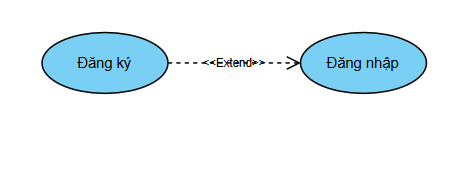
\includegraphics[width=0.45\linewidth]{figures/c3/3-3-1-rd.png} \\ 
    \hline
\end{tabular}

% \begin{figure}[H]
%     \centering  
%     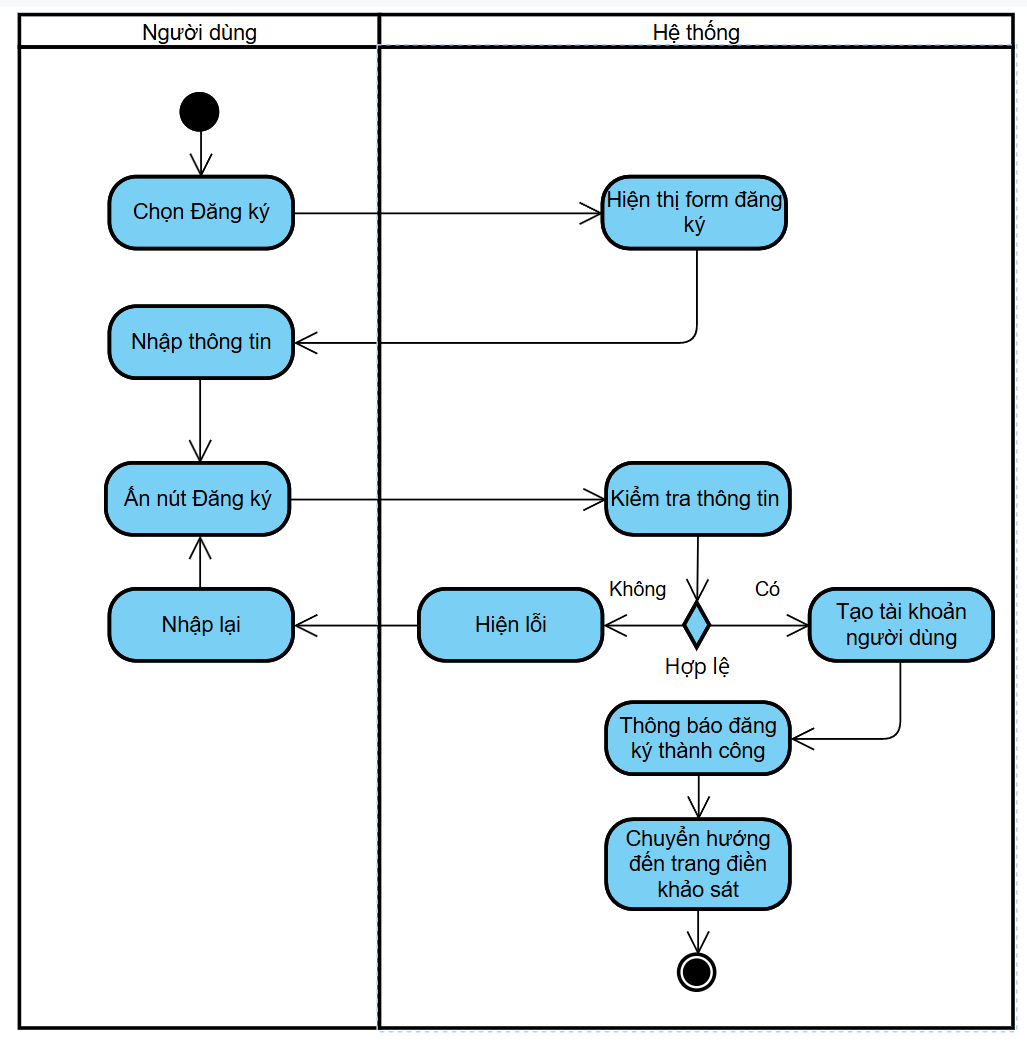
\includegraphics[width=0.5\textwidth]{figures/c3/3-3-1-ad.png}
%     \caption{Biểu đồ hoạt động ca sử dụng đăng ký.}
%     \label{fig:3-3-2-activity-diagram}
% \end{figure}



\begin{figure}[H]
    \centering  
    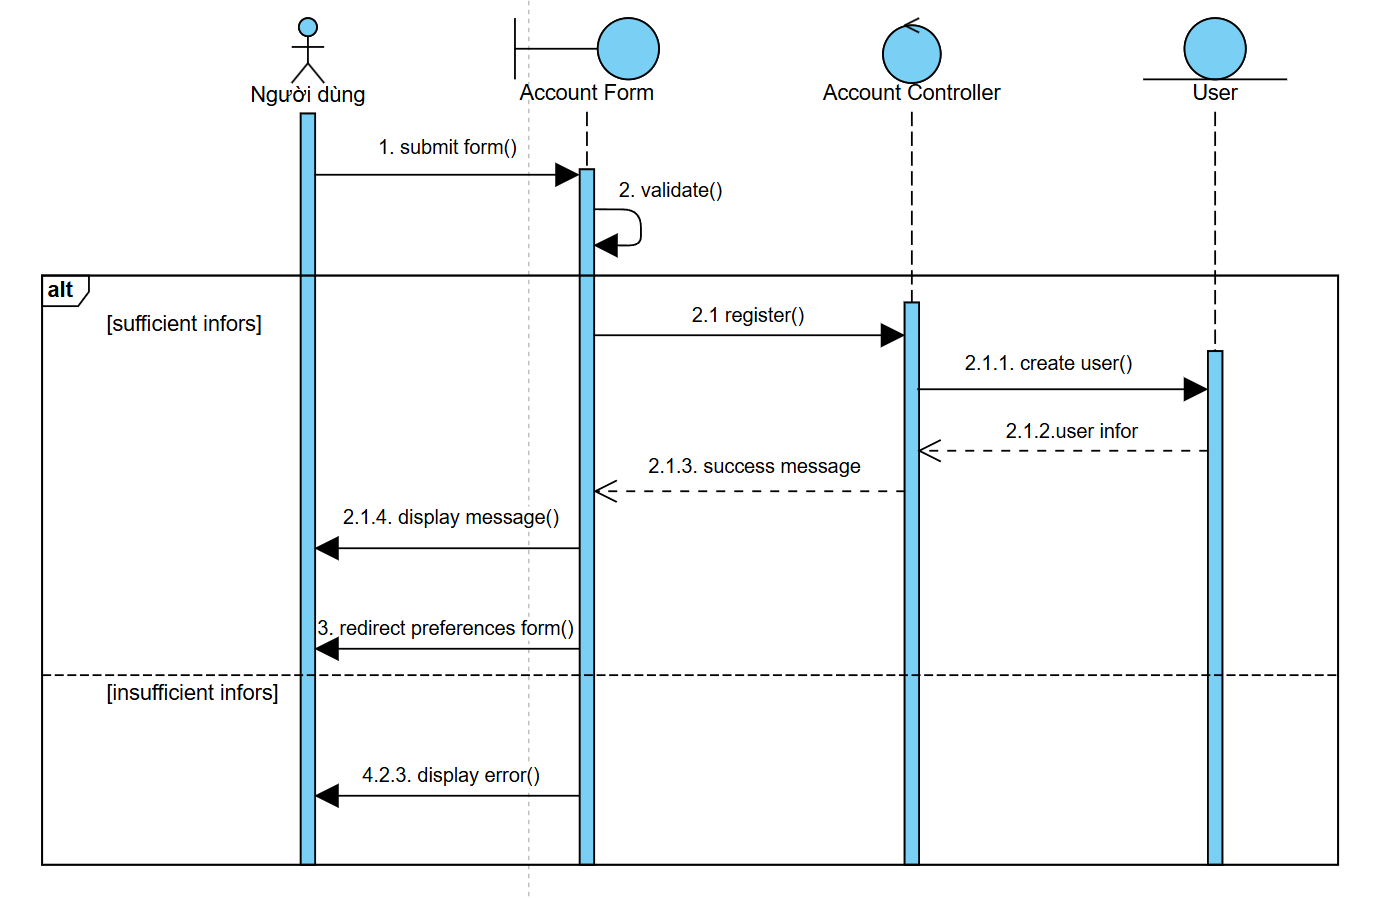
\includegraphics[width=1.05\textwidth]{figures/c3/3-3-1-sd.png}
    \caption{Biểu đồ tuần tự ca sử dụng đăng ký.}
    \label{fig:3-3-2-sequence-diagram}
\end{figure}
\nopagebreak
\subsection{Ca sử dụng đăng nhập}
\vspace{0.5cm}

\noindent 
\begin{tabularx}{\linewidth}{| l | X |} 
\hline 
\textbf{Mô tả} & Khi người dùng muốn sử dụng các chức năng yêu cầu quyền đăng nhập. \\ 
\hline 
\textbf{Luồng cơ bản} & 1. Truy cập trang đăng nhập \newline 
                      2. Nhập thông tin tài khoản (email / mật khẩu) \newline 
                      3. Điều hướng đến trang home - danh sách chuyến đi công khai. \\ 
\hline 
\textbf{Luồng thay thế} & - Nếu Người dùng nhập sai thông tin tài khoản hệ thống sẽ thông báo lỗi trên form đăng nhập  \newline 
                       - Người dùng có tài khoản chưa có thông tin sở thích hệ thống điều hướng đến trang khảo sát sở thích \\
\hline 
\textbf{Tiền điều kiện} & Người dùng đã đăng xuất. \\ 
\hline 
\textbf{Hậu điều kiện} & Hệ thống lưu token đăng nhập vào local trên thiết bị. \\ 
\hline 
\textbf{Yêu cầu phi chức năng} & Hệ thống xử lý đăng nhập không quá 2s. \\ 
\hline 
\end{tabularx}

\vspace{0.8cm}

\noindent 
\begin{tabular}{| c | c |}
    \hline
    \textbf{Biểu đồ hoạt động} & \textbf{Quan hệ} \\ 
    \hline
    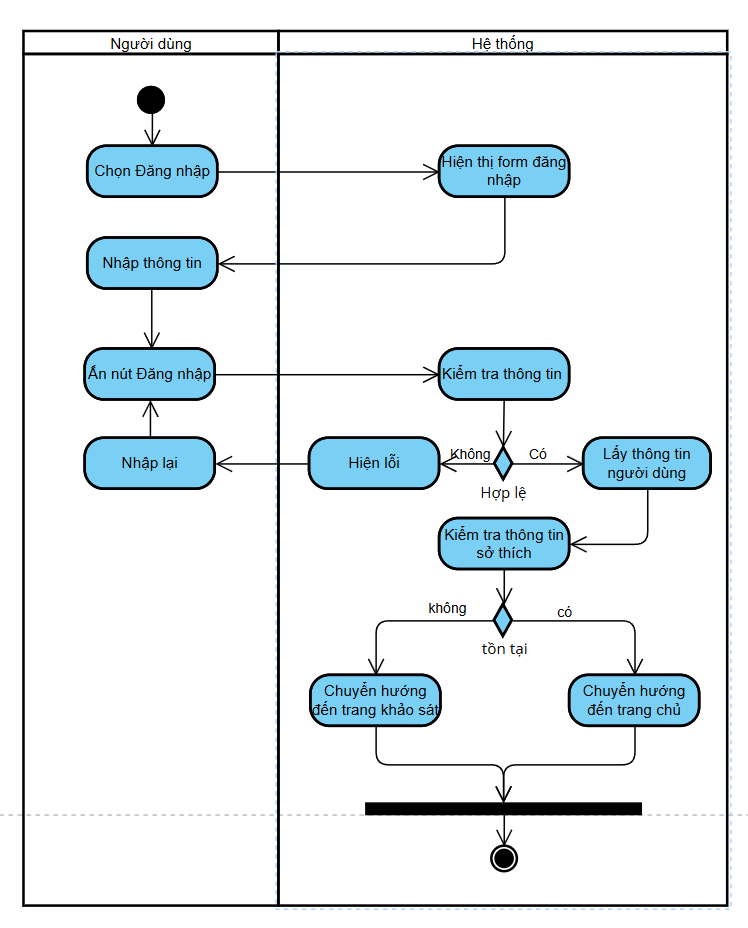
\includegraphics[width=0.5\linewidth]{figures/c3/3-3-2-ad.png} 
    & 
    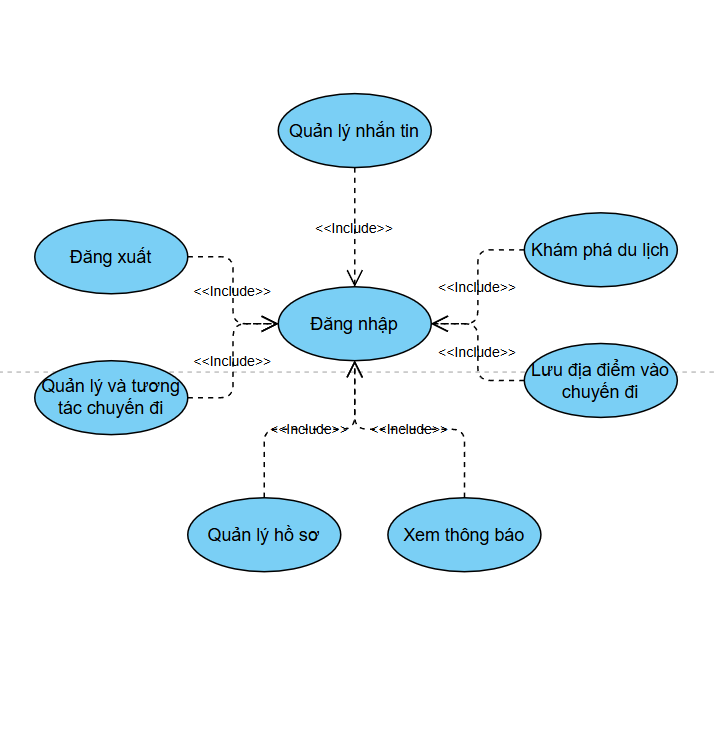
\includegraphics[width=0.45\linewidth]{figures/c3/3-3-2-rd.png} \\ 
    \hline
\end{tabular}
\vspace{0.8cm}

\begin{figure}[H]
    \centering  
    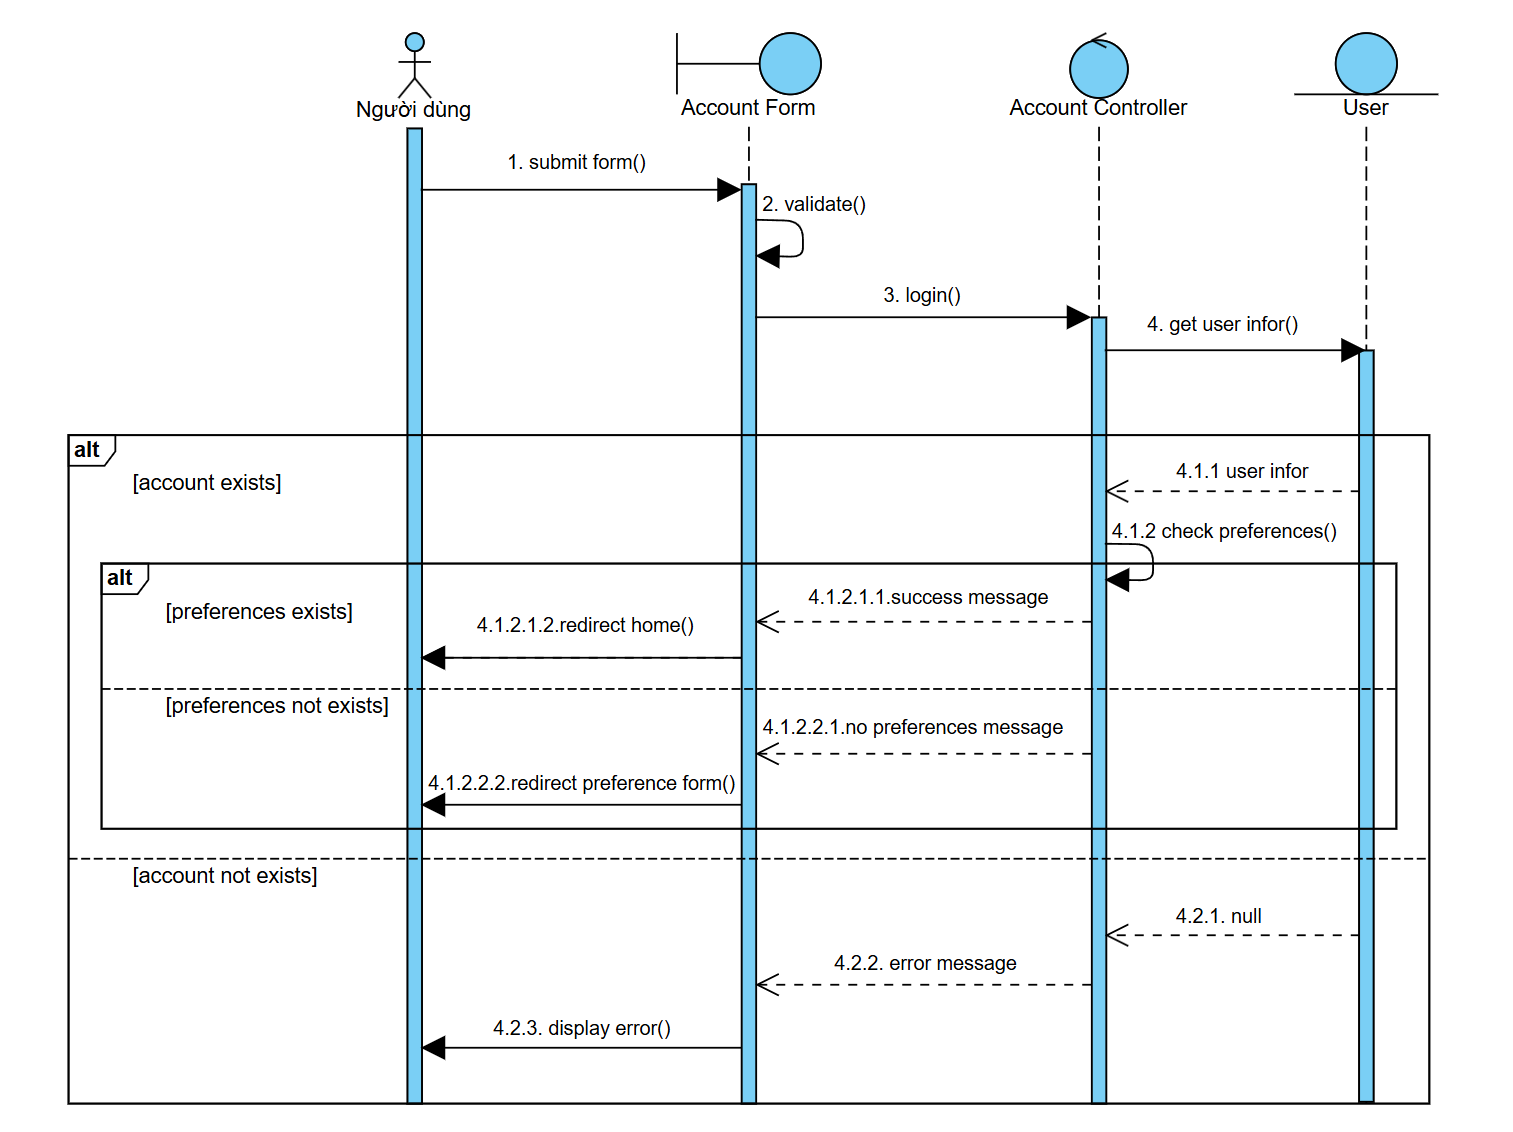
\includegraphics[width=1.05\textwidth]{figures/c3/3-3-2-sd.png}
    \caption{Biểu đồ tuần tự ca sử dụng đăng nhập.}
    \label{fig:3-3-1-sequence-diagram}
\end{figure}
\nopagebreak
\subsection{Ca sử dụng điền khảo sát sở thích}
\noindent Ca sử dụng này mô tả quá trình người dùng cung cấp thông tin về sở thích du lịch của mình sau khi đăng ký tài khoản. Thông tin này sẽ được hệ thống sử dụng để cá nhân hóa các gợi ý và trải nghiệm trong ứng dụng. Bảng~\ref{tab:uc_survey_spec} trình bày chi tiết đặc tả ca sử dụng, bao gồm luồng sự kiện chính, các điều kiện và yêu cầu liên quan. Các biểu đồ hoạt động, quan hệ (Bảng~\ref{tab:uc_survey_diagrams}) và tuần tự (Hình~\ref{fig:3-3-3-sequence-diagram}) minh họa rõ hơn về quy trình và tương tác hệ thống.

\begin{longtable}{| p{4cm} | p{\dimexpr\linewidth-4cm-4\tabcolsep} |} % Adjust widths as needed
    \caption{Đặc tả ca sử dụng điền khảo sát sở thích.} % Caption inside longtable
    \label{tab:uc_survey_spec} \\ % Label after caption

    \hline
    \textbf{Mô tả} & Người dùng cập nhật thông tin về sở thích du lịch của bản thân để sử dụng dịch vụ gợi ý trong ứng dụng \\
    \hline
    \endfirsthead % Header for the first page

    \hline
 
    \textbf{Mô tả} & Người dùng cập nhật thông tin về sở thích du lịch của bản thân để sử dụng dịch vụ gợi ý trong ứng dụng. \\
    \hline
    \endhead

    \hline 
    \endfoot

    \hline % Footer for the last page
    \endlastfoot

    \textbf{Luồng cơ bản} & 1. Người dùng đăng ký tài khoản mới \newline
                           2. Ứng dụng hiển thị các form lựa chọn lần lượt theo loại hình du lịch, giá tiền,v.v. \newline
                           3. Người dùng chọn các loại hình du lịch theo sở thích. \newline
                           4. Người dùng chọn khoảng giá du lịch phù hợp với bản thân. \newline
                           5. Người dùng nhấn nút hoàn tất để hoàn thành quá trình. \newline
                           6. Hệ thống điều hướng người dùng đến trang chủ của ứng dụng. \\
    \hline
    \textbf{Tiền điều kiện} & Người dùng đăng ký tài khoản thành công và chưa hoàn thành điền khảo sát sở thích. \\
    \hline
    \textbf{Hậu điều kiện} & Thông tin sở thích được lưu lại trong cơ sở dữ liệu. \\
    \hline
    \textbf{Yêu cầu phi chức năng} & Hệ thống xử lý cập nhật không quá 1s \\

\end{longtable}

\begin{table}[H] % Add table environment
    \centering
    \caption{Biểu đồ hoạt động và quan hệ ca sử dụng điền khảo sát sở thích} % Add caption
    \label{tab:uc_survey_diagrams} % Add label
    \begin{tabular}{| c | c |}
        \hline
        \textbf{Biểu đồ hoạt động} & \textbf{Quan hệ} \\
        \hline
        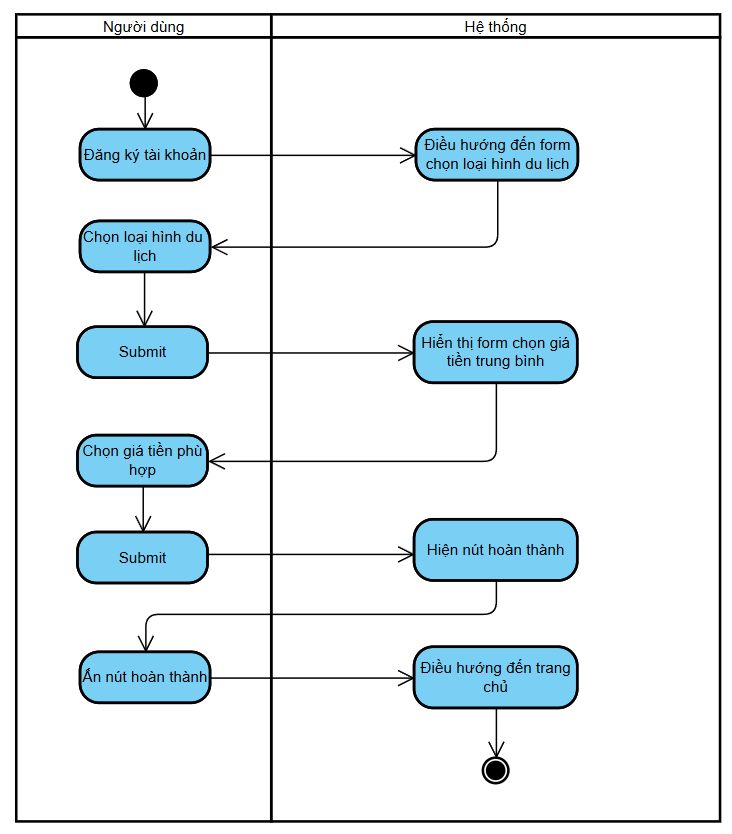
\includegraphics[width=0.5\linewidth]{figures/c3/3-3-3-ad.png}
        &
        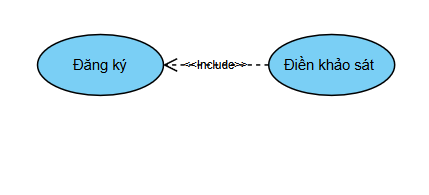
\includegraphics[width=0.45\linewidth]{figures/c3/3-3-3-rd.png} \\
        \hline
    \end{tabular}
\end{table}


\begin{figure}[H]
    \centering
    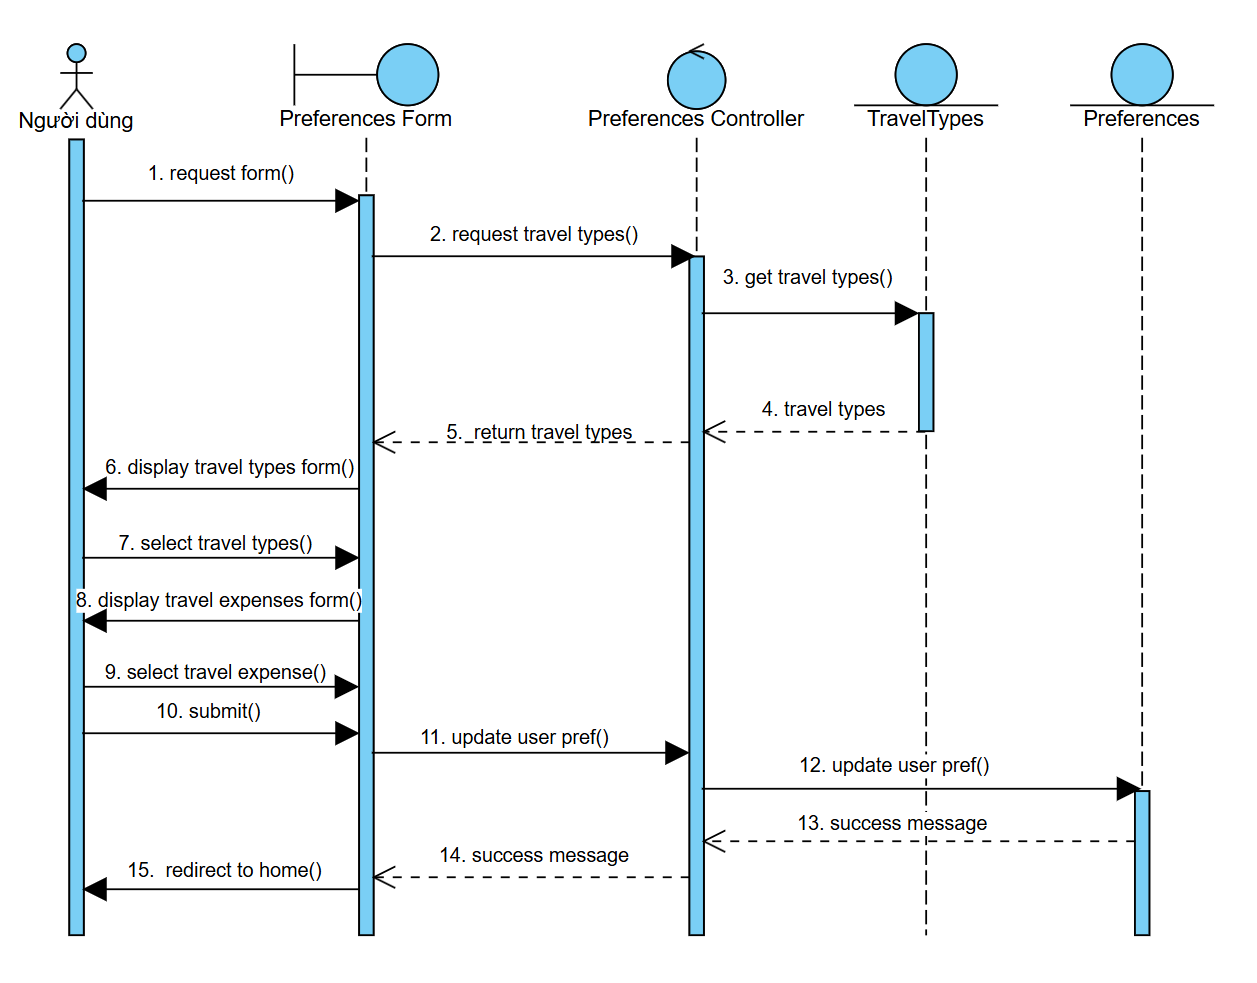
\includegraphics[width=0.85\textwidth]{figures/c3/3-3-3-sd.png}
    \caption{Biểu đồ tuần tự ca sử dụng điền khảo sát sở thích.}
    \label{fig:3-3-3-sequence-diagram}
\end{figure}
\nopagebreak
% \input{chapters/c3/usecases/3.3.4_usecase}
% \nopagebreak
% \input{chapters/c3/usecases/3.3.5_usecase}
% \nopagebreak
% \input{chapters/c3/usecases/3.3.6_usecase}
% \nopagebreak
% \input{chapters/c3/usecases/3.3.7_usecase}
% \nopagebreak
% \input{chapters/c3/usecases/3.3.8_usecase}
% \nopagebreak
% \input{chapters/c3/usecases/3.3.9_usecase}
% \nopagebreak
% \input{chapters/c3/usecases/3.3.10_usecase}
% \nopagebreak
% \input{chapters/c3/usecases/3.3.11_usecase}
% \nopagebreak
% \input{chapters/c3/usecases/3.3.12_usecase}
% \nopagebreak
% \input{chapters/c3/usecases/3.3.13_usecase}
% \nopagebreak
% \input{chapters/c3/usecases/3.3.14_usecase}
% \nopagebreak
% \input{chapters/c3/usecases/3.3.15_usecase}
% \nopagebreak
% \input{chapters/c3/usecases/3.3.16_usecase}
% \nopagebreak
% \input{chapters/c3/usecases/3.3.17_usecase}\nopagebreak